\chapter[Modulating metabolic state]{ Carbon substrate dependent variation of metabolic state in budding yeast}\label{ch:three}
\clearpage
\section{Introduction}
Budding yeast are able to generate their energy from either fermentation or respiration. When grown in conditions where they are forced to undergo respiration, their mitochondrial networks display an increase in size and appear more connected ('degree of ramification', \cite{jakobs_spatial_2003}). This simple but powerful connection between metabolic state and morphology of the organelle underlies our rationale for varying growth substrates to study the structure-function relationship in yeast mitochondrial networks. We begin this chapter with an overview of how yeast metabolize different carbon substrates using either fermentation or respiration dependent pathways, how cellular respiration and oxidative phosphorylation (OXPHOS) respond to bioenergetic needs of the cell, how we might measure the bioenergetic state of cells and what the expected levels of these measurements would be for the substrates we used in this study.

The preferred sugar sources of budding yeast are glucose and fructose \cite{bergman_growth_2001}. When glucose levels are high, the expression of enzymes and proteins needed for metabolizing other types of carbon sources and mitochondrial biogenesis are repressed and all energy is derived via fermentation. This phenomenon is known as carbon catabolite repression or alternatively glucose repression \cite{gancedo_yeast_1998}.Yeast can utilize non-fermentable carbon sources such as ethanol, pyruvate, lactate and glycerol. Yeast grown under aerobic conditions on these substrates derive their cellular energy almost exclusively from respiration \cite{fendt_transcriptional_2010}. The oxidation of pyruvate to acetyl-CoA generates one unit of the reducing agent NADH. Acetyl-CoA then serves as a substrate for further oxidation in the tricarboxylic acid (TCA) cycle. Lactate is oxidized to pyruvate by an external, intermembrane facing complex known as \emph{lactate:cytochrome c} oxidoreductase, located near the end of the electron transport chain (ETC) \cite{pajot_utilization_1974}. Ethanol is converted to acetyl-CoA via the NAD+ dependent alcohol dehydrogenases, generating two units of NADH \cite{luttik_saccharomyces_1998,wills_regulation_1990}. Glycerol is converted to glyceraldehyde-3-phosphate, an intermediate metabolite in the glycolysis pathway which ultimately generates pyruvate. Gycerol also plays a role in the glycerol-3-phosphate shuttle which allows cytosolic NADH to provide the electrons directly into the ETC \cite{larsson_importance_1998}.

NADH is oxidized aerobically in the mitochondria by donating electrons into the ETC chain. Oxidation of NADH in the OXPHOS process generates around 1.5 ATP units of \cite{ouhabi_flux-yield_1989}. This stoichiometry is lower than other higher eukaryotes (commonly given as 2.5 ATP per NADH) due to the fact that the NADH dehydrogenase (Complex I equivalent) in yeast is non proton translocating, resulting in a lower ATP/oxygen conversion ratio. In mammalian cells, NADH donates electrons into the chain solely through the internal (matrix facing) NADH dehydrogenase Complex I. However yeast also have external (intermembrane facing) dehydrogenases Nde1p/Nde2p \cite{luttik_saccharomyces_1998}. This means that substrates that are not derived from the TCA cycle can also contribute to cellular respiration. An example of this is the pyruvate dehydrogenase bypass \cite{boubekeur_mitochondrial_1999}, where pyruvate oxidation occurs in the cytosol and the NADH generated from cytosolic pyruvate oxidation is reoxidized via these external dehydrogenases. The net result is that the ATP yield from pyruvate catabolism is lower than would be expected in yeast. 

Yeast can also utilize fermentable non repressing carbon sources, such as raffinose and galactose. Under these conditions both fermentation and respiration can occur simultaneously. Raffinose is a trisaccharide composed of glucose, fructose and galactose. Raffinose is hydrolyzed to fructose and melibiose, a disaccharide consisting of glucose and galactose \cite{paulo_proteome-wide_2015}. Galactose is converted to glucose-6-phosphate via the Leloir Pathway and then enters the glycolysis pathway, ultimately generating pyruvate which enters the TCA cycle.

\subsection{Parameters of the OXPHOS process}
The main physiological role of mitochondria in the cell is ATP generation by OXPHOS. In the context of this project, our main interest is related to the function of the respiratory chain of the mitochondria. Therefore the most relevant assays are those related to cellular respiration and maintenance of the proton motive force (PMF), which are critical parameters of the OXPHOS process. 
%
\begin{figure}[htp]
	\centering
    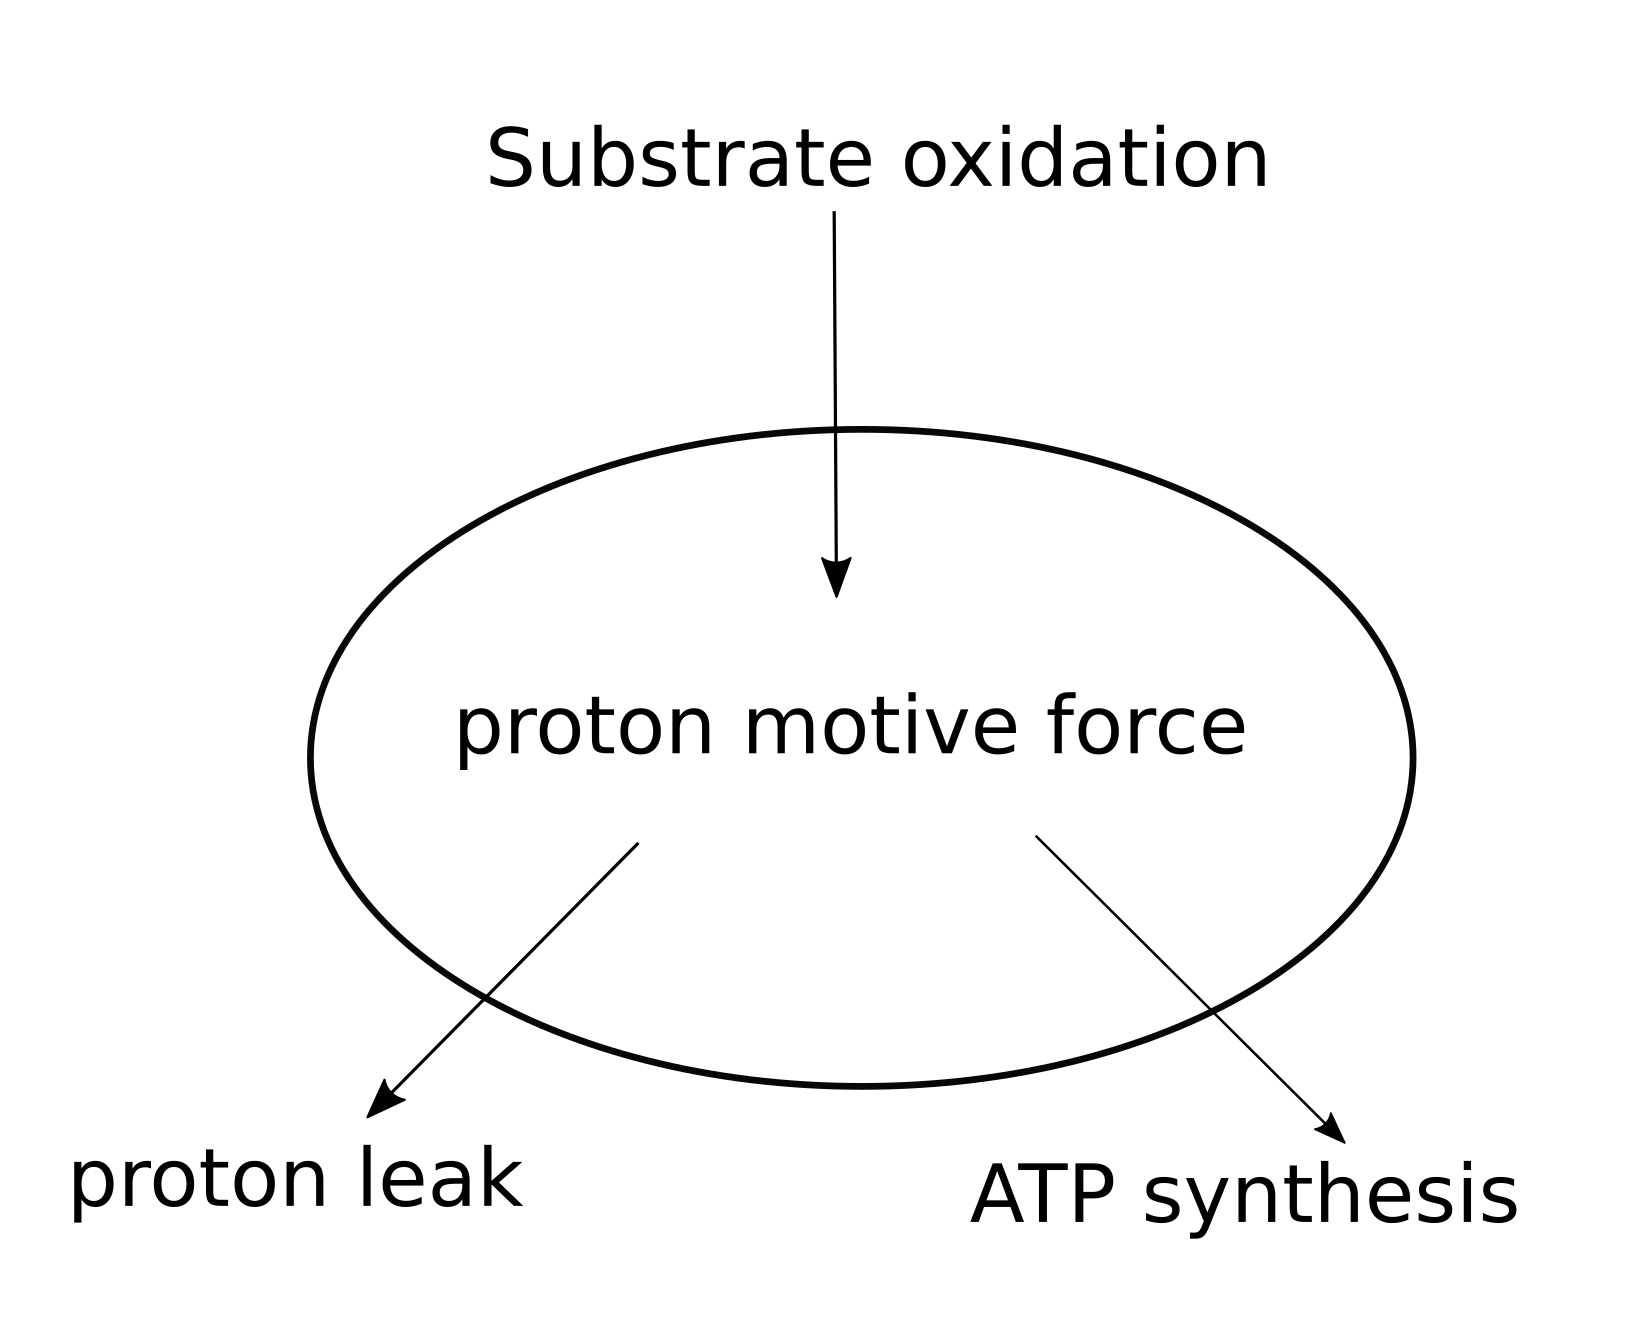
\includegraphics[width=.5\textwidth]{device}
    \caption[Components of OXPHOS respiration]{Substrate oxidation driven respiration generates proton motive force which is consumed by ATP synthesis and proton leak.\\Substrate oxidation consists of all reactions upstream of the ATP synthase, such as reactions in the ETC and those involved in substrate uptake mechanisms. ATP synthesis occurs via OXPHOS at the ATP synthase complex while proton leak consist of all reaction that consume PMF and do not generate ATP.}\label{fig:device}
\end{figure}
%

The respiratory chain of the mitochondria consists of the electron transport chain (ETC) and OXPHOS protein complexes. If we consider the ETC/OXPHOS component of the mitochondria as the 'device' (\Fref{fig:device}), we can think of the input into the device as the rate of metabolic substrate oxidation which generates the PMF. The device than uses PMF to generate ATP via phosphorylation of ADP. There are losses and shunts in the system due to proton leak, which consumes PMF but does not result in ATP synthesis. The current into this device is measured via the respiration rate. Mitochondrial respiration rate is directly related to the amount of oxygen been reduced to water at Complex IV, the terminal end of the ETC cascade. Because of the tight coupling \cite{hafner_effect_1991} between electrons entering the ETC cascade and protons pumping out of the matrix, oxygen consumption measures the proton current flowing in the ETC cascade. Proton motive force (PMF), which is composed mainly of ΔΨ \eqref{eq:pmf} is a measure of the electrochemical gradient available to drive ATP synthesis and is analogous to the voltage level of a device. Together these two assays (O$_2$ consumption and measurement of PMF/ΔΨ levels) are able to give a quantitative assessment of mitochondrial functional state \cite{brand_assessing_2011}.
%
\begin{equation}\label{eq:pmf}
\text{PMF}=\mupDelta\mupPsi-61.5\text{ΔpH}
\end{equation}

\Fref{fig:pmfo2} gives an excellent summary of how the input, output and losses/shunts of the ETC/OXPHOS machinery are related to the current-voltage characteristics of the system. As we move toward the left along the red curve (increasing substrate oxidation rate, state 4 to state 3), respiration rate rises steeply as PMF is consumed. At this maximal respiration rate (state 3, ADP present with substrate), the response of ATP synthesis to PMF is shown in the blue curve. The respiration rate is progressively inhibited via a substrate enzyme inhibitor (malonate). This blue curve shows that the amount of PMF generated is a linear function of the amount of respiration. The 'proton leak' (green curve) is similarly derived by progressively inhibiting substrate oxidation at state 4 (no ADP). PMF gradually falls as proton leak driven respiration goes to zero. This also brings up an important point of proton leak respiration: even when there is no ATP synthesis activity, endogenous substrate driven respiration still occurs to generates a PMF that is then consumed by the proton leak shunt. In other words the mitochondrial machinery keeps the respiration machinery primed with PMF to respond to a change in ATP demand. The relative proportion of respiration been consumed by ATP synthesis and proton leak as a function of respiration levels and substrate oxidation rate is shown in \Fref{fig:respratios}.

\Fref{fig:pmfo2} and \Fref{fig:respratios} show that OXPHOS is a complex process that is affected by many factors. There are therefore many ways to measure the state of OXPHOS driven respiration. The next two sections will focus on two parameters that are used to measure OXPHOS respiration in this project.

\begin{figure}[htp]
	\centering
    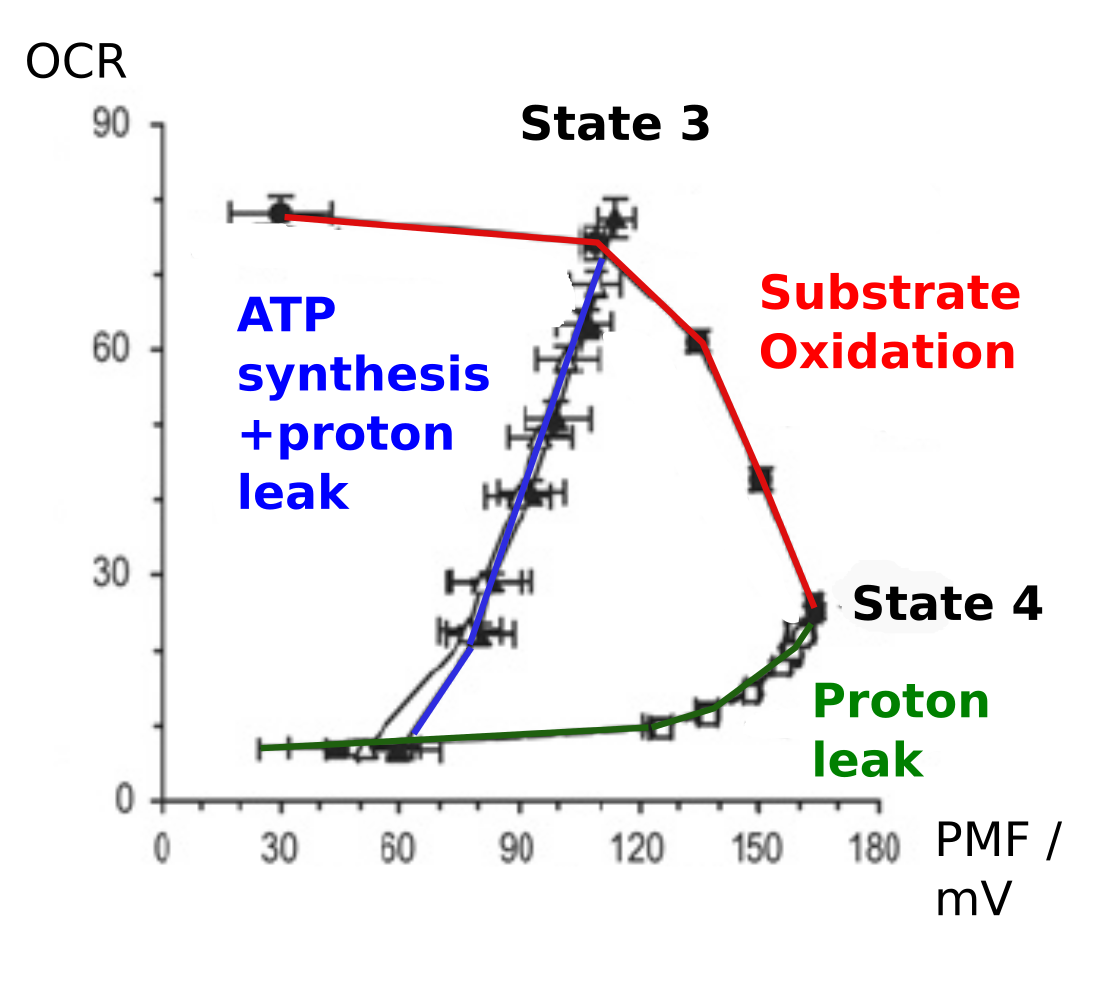
\includegraphics[width=.7\textwidth]{pmfo2}
    \caption[Respiration – PMF relationship of mitochondria]{Respiration – PMF relationship of mitochondria isolated from human lung carcinoma cells.\\Shown is response curve of substrate oxidation, proton leak respiration and ATP synthesis to PMF. The substrate given was succinate. Respiration levels were modulated via titration of FCCP for the substrate oxidation curve and malonate titration for the ATP synthesis and proton leak curves. State 3 (maximal respiration, ADP present) and State 4 (minimal respiration, no ADP) are indicated in the substrate oxidation curve. Note the linear relationship between respiration rate and PMF consumed during ATP synthesis (blue line).\\\emph{Adapted from Figure 2B of Brand et al., "Assessing mitochondrial dysfunction in cells", Biochem J 2011, used under CC BY-NC 2.5}}\label{fig:pmfo2}
\end{figure}
%
\begin{figure}[htp]
	\centering
    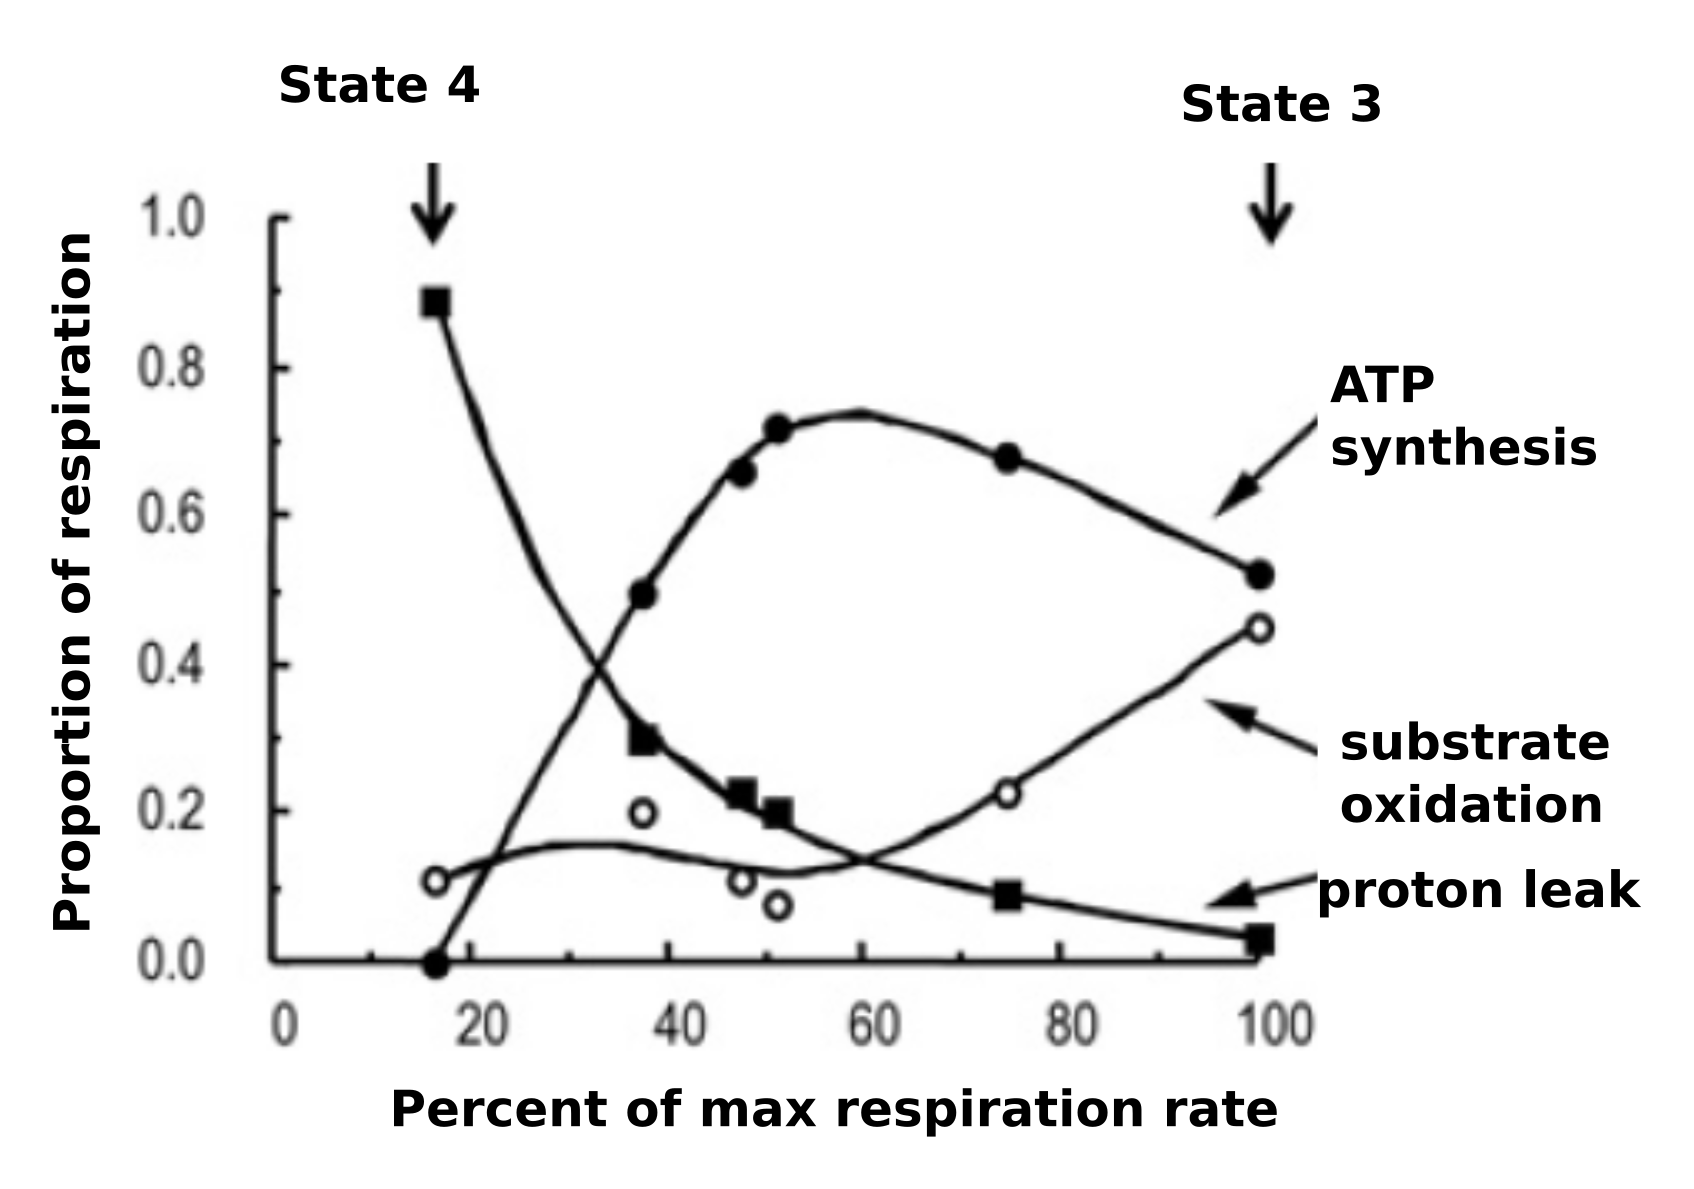
\includegraphics[width=.7\textwidth]{respratios}
    \caption[Proportion of respiration from the input and outputs of ETC/OXPHOS]{Proportion of respiration from the input and outputs of ETC/OXPHOS.\\At different respiration levels, the amount of proton leak varies depending on the level of ATP synthesis. Proton leak is maximal when ATP synthesis is zero, to maintain PMF equilibrium generated by substrate oxidation.\\\emph{Adapted from Figure 2C of Brand et al., "Assessing mitochondrial dysfunction in cells", Biochem J 2011, used under CC BY-NC 2.5}}\label{fig:respratios}
\end{figure}
%
\subsection{Mitochondrial membrane potential (ΔΨ) as a bioenergetic indicator}
Mitochondrial membrane potential (ΔΨ) is an indicator of the electrochemical gradient that is available to drive protons from the intermembrane space (IMS) into ATP synthase to phosphorylate ADP to ATP. Although respiration levels have a large gradient in relation to PMF (a large change in respiration levels results in a small PMF/ΔΨ change (\Fref{fig:pmfo2}, red curve); the use of ΔΨ as a bioenergetic indicator is still relevant. Whereas respiration measurements can only be done at a bulk level, ΔΨ measurements using fluorescent lipophilic dyes that accumulate in a Nernstian manner enable direct visualization of ΔΨ at the level of individual mitochondria \cite{twig_tagging_2006,wikstrom_-cell_2007}. In addition, mitochondrial dynamics, in particular selective fusion of mitochondrial fragments are believed to be dependent on ΔΨ \cite{twig_fission_2008}. Since fusion is believed to be affected by ΔΨ levels, one can use ΔΨ as a biomarker for function and correlate it with changes to the structure of the mitochondrial network. 
\subsection{Oxygen consumption measurement of cellular respiration}
The classic assay for cell respiration was developed by Chance and Williams \cite{chance_respiratory_1955}, using a Clark electrode to measure oxygen consumption rate (OCR) in isolated mitochondria. In this assay, isolated mitochondria are incubated with a substrate and ADP (state 3). As respiration increases the dissolved oxygen concentration decreases. The reduction of oxygen to water by the flow of electrons from the ETC generates the necessary PMF for ATP synthesis. Once ATP/ADP levels reach an equilibrium, ATP synthesis and respiration rates slow down (state 4).
%
\begin{figure}[htp]
	\centering
    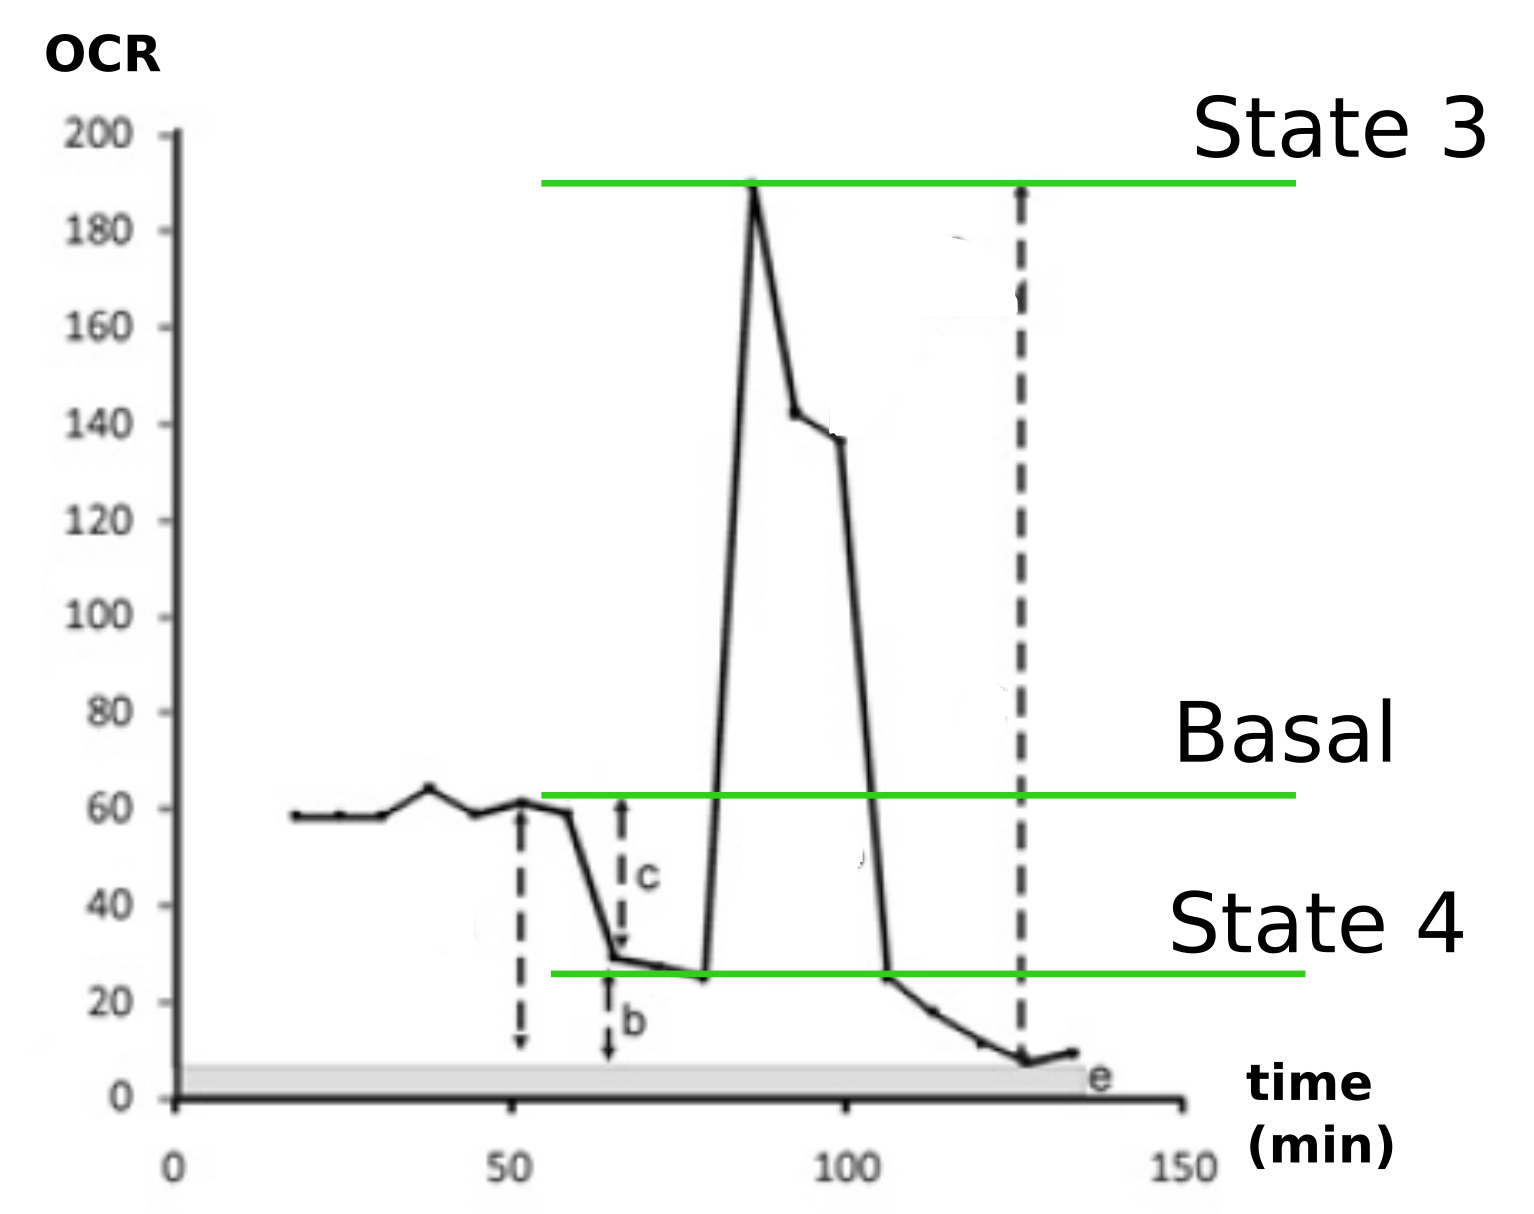
\includegraphics[width=.65\textwidth]{basal}
    \caption[Definition of State 3, basal and State 4 respiration levels]{State 3, basal and State 4 respiration levels in rat cortical neuron cells.\\State 4 is reached by addition of oligomycin from basal respiration levels. State 3 is reached by addition of a protonophore, FCCP from State 4. Respiratory control ratio is the ratio of state 3 to state 4 respiration level, spare respiratory capacity is State 3 minus basal level respiration.\\\emph{Adapted from Figure 3A of Brand et al., "Assessing mitochondrial dysfunction in cells", Biochem J 2011, used under CC BY-NC 2.5}}\label{fig:basal}
\end{figure}
%

In intact cells, state 3 can be approximated by the addition of a protonophore such as FCCP, to allow uncoupled (not tied to OXPHOS) maximal respiration (\Fref{fig:basal}). State 4 can be approximated by the addition of oligomycin to inhibit the ETC cascade. Any respiration detected in state 4 is due to 'leak' respiration (respiration due to protons reentering directly into the matrix). We used the Clark electrode method to measure basal respiration in this study. In intact cells, basal respiration corresponds to a state intermediate between State 3 (unlimited substrate and ADP, maximum respiration) and State 4 (unlimited substrate, no ATP synthesis, minimal respiration).
\subsection{Variation of carbon source substrates and their expected bioenergetic measurements}\label{sec:carbon}
In the context of this project, we wanted to study the change of structure and function in the mitochondrial network in one metabolic state (fermentation) compared to another (respiration). Therefore we grew yeast cells in different carbon sources to obtain:
\begin{enumerate}[label=\emph{\alph*}), leftmargin=*, itemindent=0pc]
\item glucose repressing conditions (2\% glucose)
\item fermentable, non repressing conditions (2\% raffinose)
\item Non-fermentable carbon substrates (2\% lactate and 2\% glycerol + 2\% ethanol). The use of two different non-fermentable carbon substrates was due to the fact that glycerol enters the glycolytic pathway, and though it is usually considered a non-fermentable substrate we decided to include lactate which completely bypasses the glycolytic pathway. 
\end{enumerate}
Based on the above review and our understanding of how each of the different carbon sources are metabolized, we expected cells grown in glucose to have the lowest OCR and ΔΨ due to the glucose repression effect. The non-fermentable carbon substrates (lactate and glycerol+ethanol) were expected to have the highest OCR and ΔΨ due to the cells having to undergo aerobic respiration. Raffinose was expected to have intermediate levels of OCR and ΔΨ as it is able to undergo simultaneous fermentation and respiration.
\section{Materials and Methods}
\subsection{\texorpdfstring{O\textsubscript{2}}{O2} consumption rate measurement using a Clark electrode}
The Clark type electrode measures oxygen on a catalytic platinum surface \cite{li_measurement_2012}. The system consists of a platinum cathode and silver anode, bridged by a potassium chloride electrolyte (\Fref{fig:clark}). An oxygen permeable membrane separates the electrode from a sealed chamber containing the liquid sample to be measured. The platinum cathode is reduced by oxygen diffusing through the membrane. The current is proportional to the oxygen concentration in the solution. At the silver anode, the circuit is completed by the precipitation of silver chloride from the ions at the anode. An analog to digital converter unit records the current that represents the oxygen concentration in the sample.
%
\begin{figure}[htp]
	\centering
    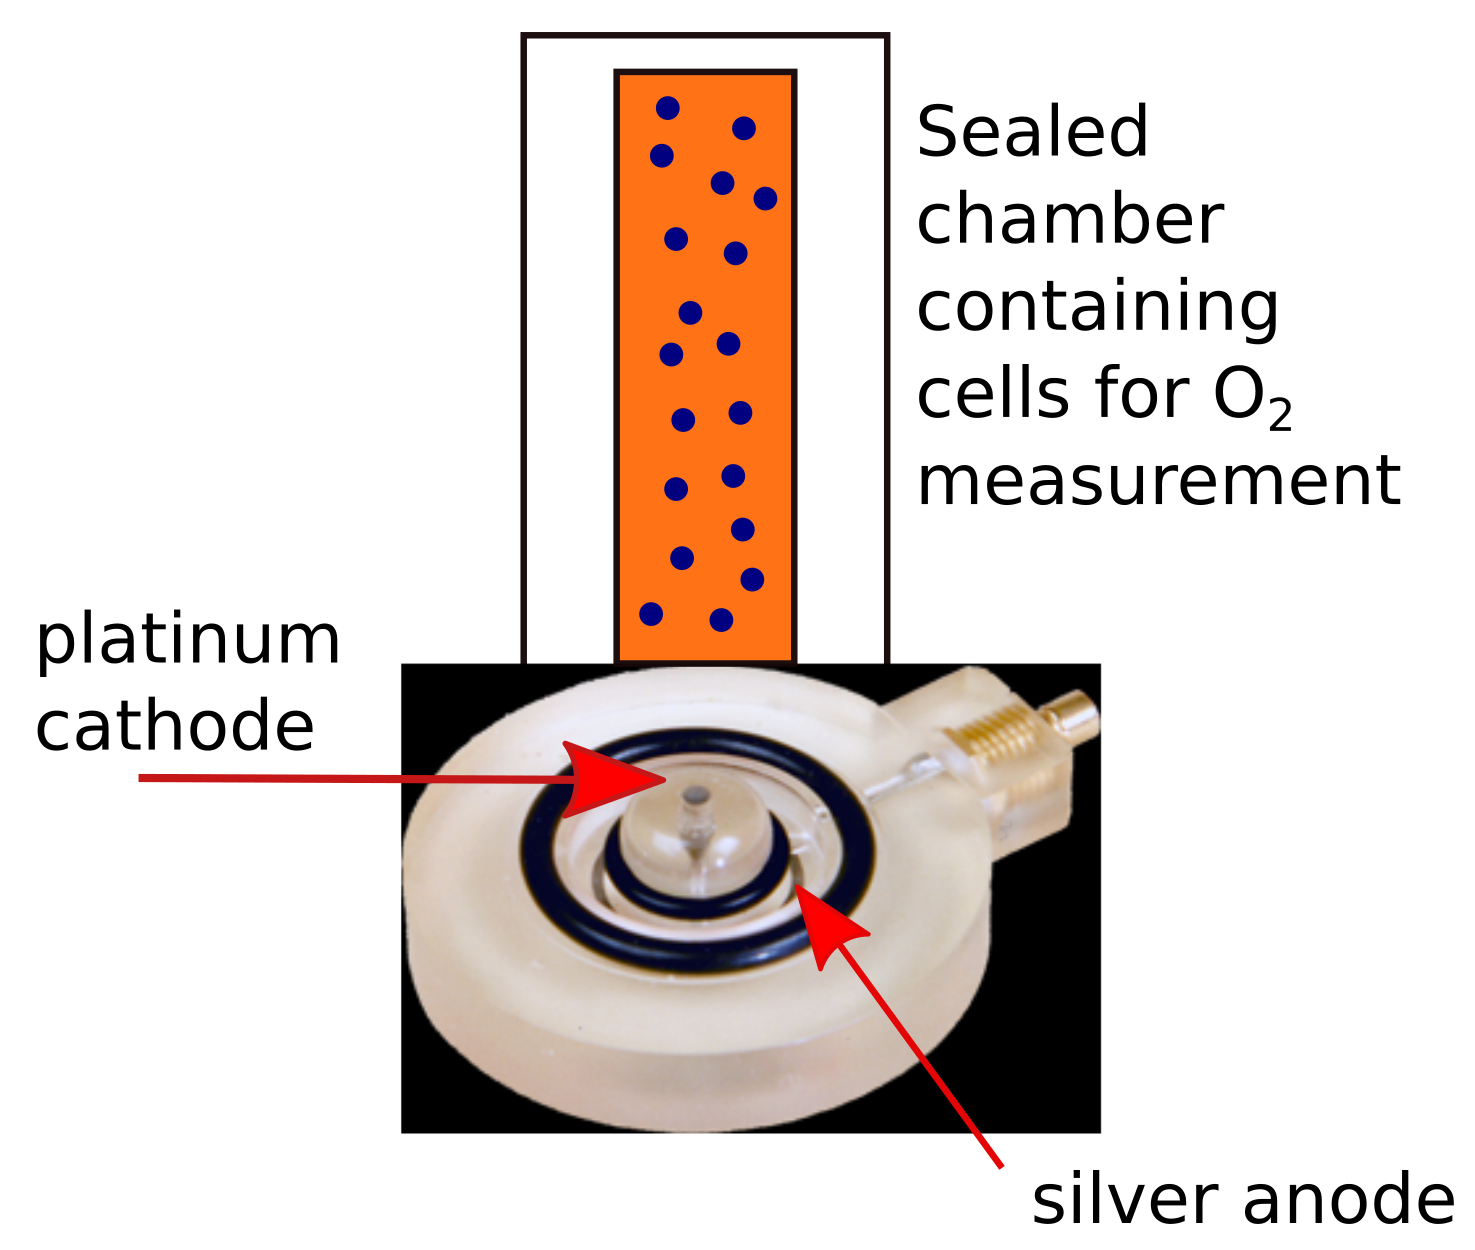
\includegraphics[width=.7\textwidth]{clark}
    \caption[Diagram of a Clark electrode used for oxygen consumption rate (OCR) measurement]{Diagram of a Clark electrode used for oxygen consumption rate (OCR) measurement.\\
A PTFE oxgyen permeable membrane covers the platinum cathode and separates the cathode from the sample. An electrolyte soaked wicking paper, which lies underneath the membrane serves as an electrolytic bridge from the cathode to the anode. The current generated at the cathode is directly proportional to the oxygen concentration in the sample (cells shown as blue dots), which is enclosed by a sealed chamber (orange and white rectangle).}\label{fig:clark}
\end{figure}
%

Oxygen consumption of yeast cells grown in the following media were measured in a Clark oxygen electrode chamber (Oxytherm, Hansatech Instruments): Yeast extract + peptone (YP) + glucose 2\% (YPD), YP + 2\% glycerol + 2\% ethanol (YPE), YP + 2\% lactate (YPL), YP + 2\% raffinose. Measurements of each condition consisted of 6--10 runs over 2 days (total N=14--20). Oxygen consumption rate (OCR) was reported as \si{\OCR}. We normalized OCR by dry weight of cell as well as by cell number and mitochondrial volume.
\subsection{OCR measurement protocols}
\begin{enumerate}[label=\arabic*), leftmargin=*, itemindent=0pc]
\item Cells were grown in suspension to log phase (details in \fref{sec:loaddye})
\item Setup and calibration of the electrode was performed on the day of the experiment using the instructions from the manufacturer. A 50\% potassium chloride solution was pipetted onto the platinum cathode and then covered with a PTFE membrane. The electrode chamber was filled with aerated water and flushed with nitrogen gas to establish a zero baseline measurement. Calibration was done at room temperature (22°C).
\item\label{itm:3} Starting from the lowest optical density (OD$_{600}$) reading (typically \textasciitilde0.25), a 1 ml cell suspension was pipetted into the electrode chamber. The reading was then taken for between 2--5 minutes. The OCR at that particular OD$_{600}$ was measured as the slope of the linear part of the curve (between the red lines in \Fref{fig:linear}) and expressed as \si{\OCR}. After every measurement the cells were aspirated and the chamber flushed with clean water.
Step \ref{itm:3} was repeated for increasing OD$_{600}$ readings up to about OD$_{600}$ of about 0.5.  The maximum OD$_{600}$ was limited by the fact that as the cell density increased in the chamber, the length of time for which a linear part of the curve can be obtained was decreased. The maximum OD$_{600}$ for each condition was around 0.5--0.6. A curve for OCR as a function of cell optical density OD$_{600}$ was then fitted (\Fref{fig:OCRraw}). The shaded bands represent the bootstrapped 95\% confidence intervals of the fitted OCR values.
\item OCR normalized to unit mass of cells was obtained by measuring the dry mass of cells at an OD$_{600}$ of approximately 0.5 for each of the experimental growth conditions. Cell mass was obtained by growing \textasciitilde{8 ml} of yeast cell culture in a weighted conical glass tubes (Corning 99502-15), to an OD$_{600}$ of approximately 0.5. The glass tube was then centrifuged for 15 minutes at 3000g to pellet the cells and the supernatant discarded. The glass tube was then oven dried at 70°C for two to three days. The glass tube was weighed again and the dry mass of cell obtained by taking the difference of the two weights, expressed as \si{\mg\per\ml} normalized to OD$_{600}$=0.5.  All dry weight measurements were repeated at least 5 times.
\item OCR was also normalized to cell number per ml at OD$_{600}$=0.5. Cell number was obtained by growing yeast cells to about OD$_{600}$=0.5. A \SI{1}{\ul} sample was placed into a hematocytometer (model 3100, Hausser Scientific, PA) and a cover slip was placed over the chamber. The counting chamber consisted of a predefined volume of liquid \SI{.1}{\ul}. The central square in the hematocytometer consisted of a volume of \SI{.004}{\ul}. The square was ruled into 25 groups, so each group held a volume of \SI{.00025}{\ul}. The cells were counted using 5 of the 25 groups in the central square. The average of these five reading were then multiplied by 250,000 to obtain a cell count per ml. This number was than normalized to the OD$_{600}$ it was taken at (\textasciitilde0.5) to obtain an average number of cells per ml per unit OD$_{600}$ reading. All cell counts were repeated at least 6 times.
\item OCR was also normalized to average mitochondrial volume for a particular growth condition. The average mitochondrial volume was calculated from MitoGraph v2.0 by taking the mean total length of the mitochondrial network for that cell condition (N\textasciitilde100) and multiplying by the cross section, assuming a constant mitochondrial tubule diameter of \SI{300}{\nm}. For all three methods of normalization (OCR normalized by dry weight, cell number and mitochondrial volume), the error bars shown in (\Fref{fig:O2bars}) represent the 95\% confidence interval obtained by bootstrapping 1000 samples of the normalized OCR measurement and the height of the bars represent the median value for the normalized OCR at OD$_{600}$=0.5.
\end{enumerate}
%
\begin{figure}[htp]
	\centering
    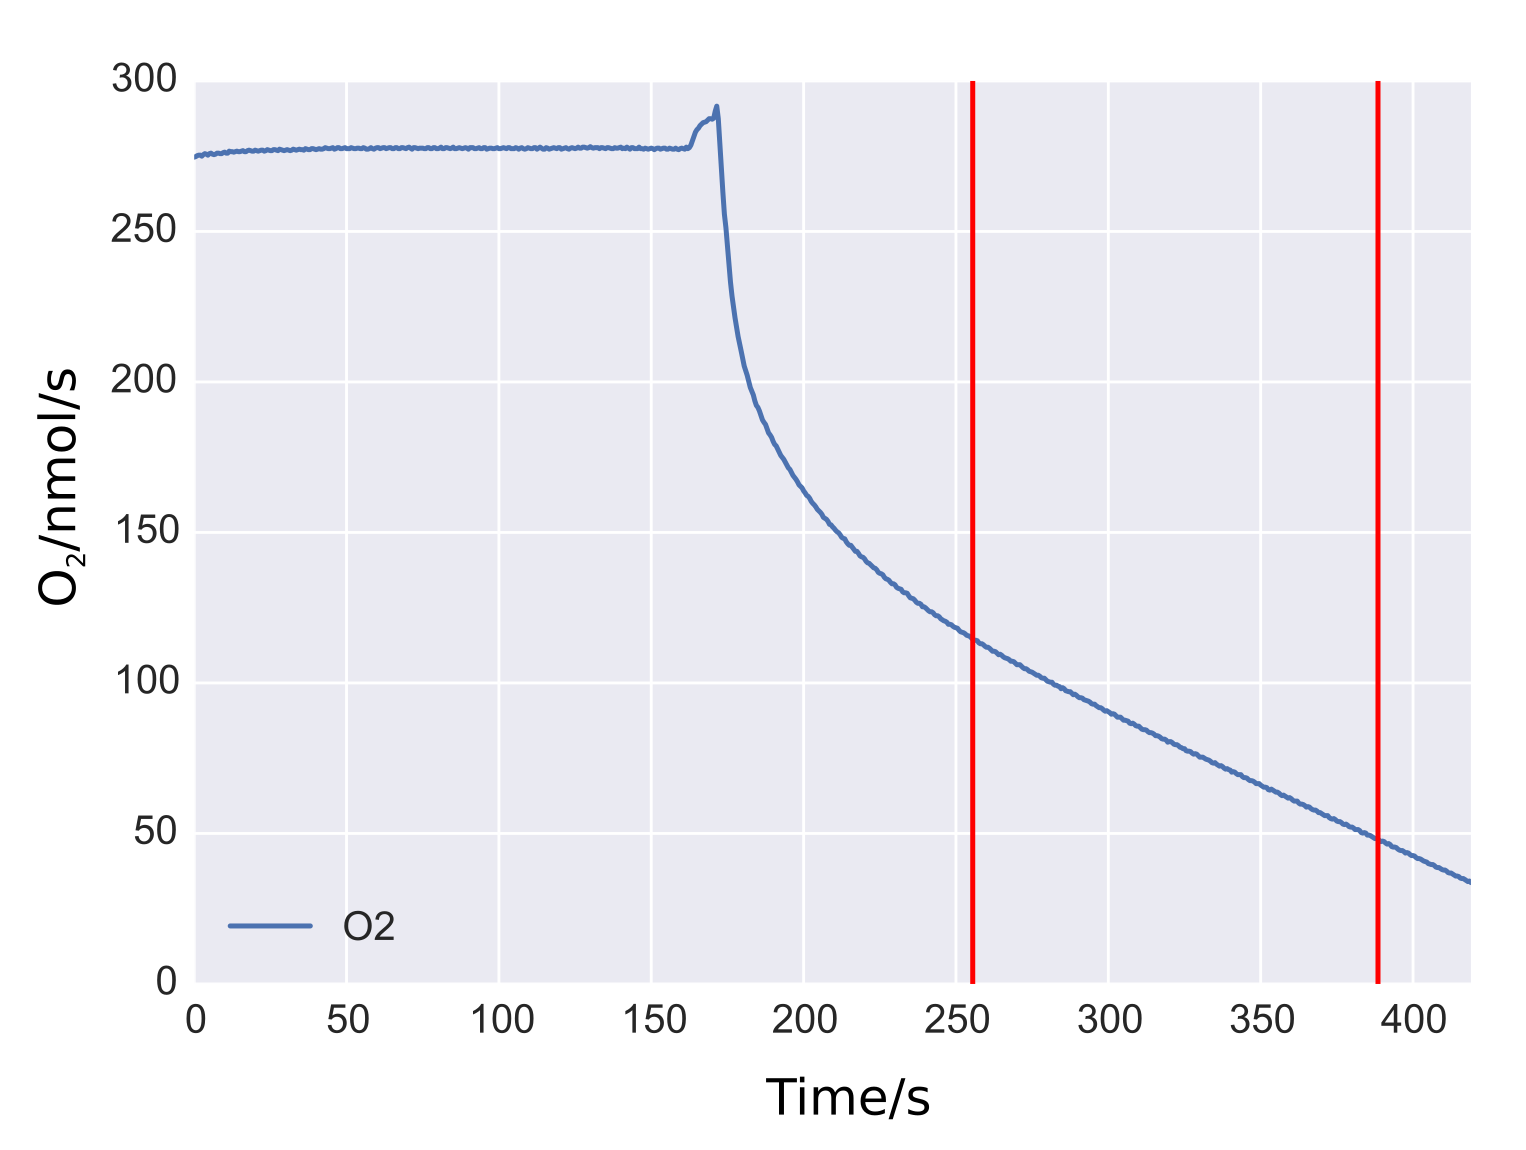
\includegraphics[width=.65\textwidth]{linear}
    \caption[Raw oxygen consumption rate (OCR) data from one sampling run at a particular carbon source and OD$_{600}$ reading.]{Raw oxygen consumption rate (OCR) data from one sampling run at a particular carbon source and OD$_{600}$ reading.\\A Clark electrode was used to measure OCR of live yeast cells grown at various concentrations (measured as optical density, OD$_{600}$). For a particular sampling run, the OCR was calculated as the slope of the linear region (between the two vertical red lines). Multiple sampling runs at different OD$_{600}$ readings are repeated to obtain the curve fit shown in \Fref{fig:OCRraw}}\label{fig:linear}
\end{figure}
%
%
\begin{figure}[htp]
	\centering
    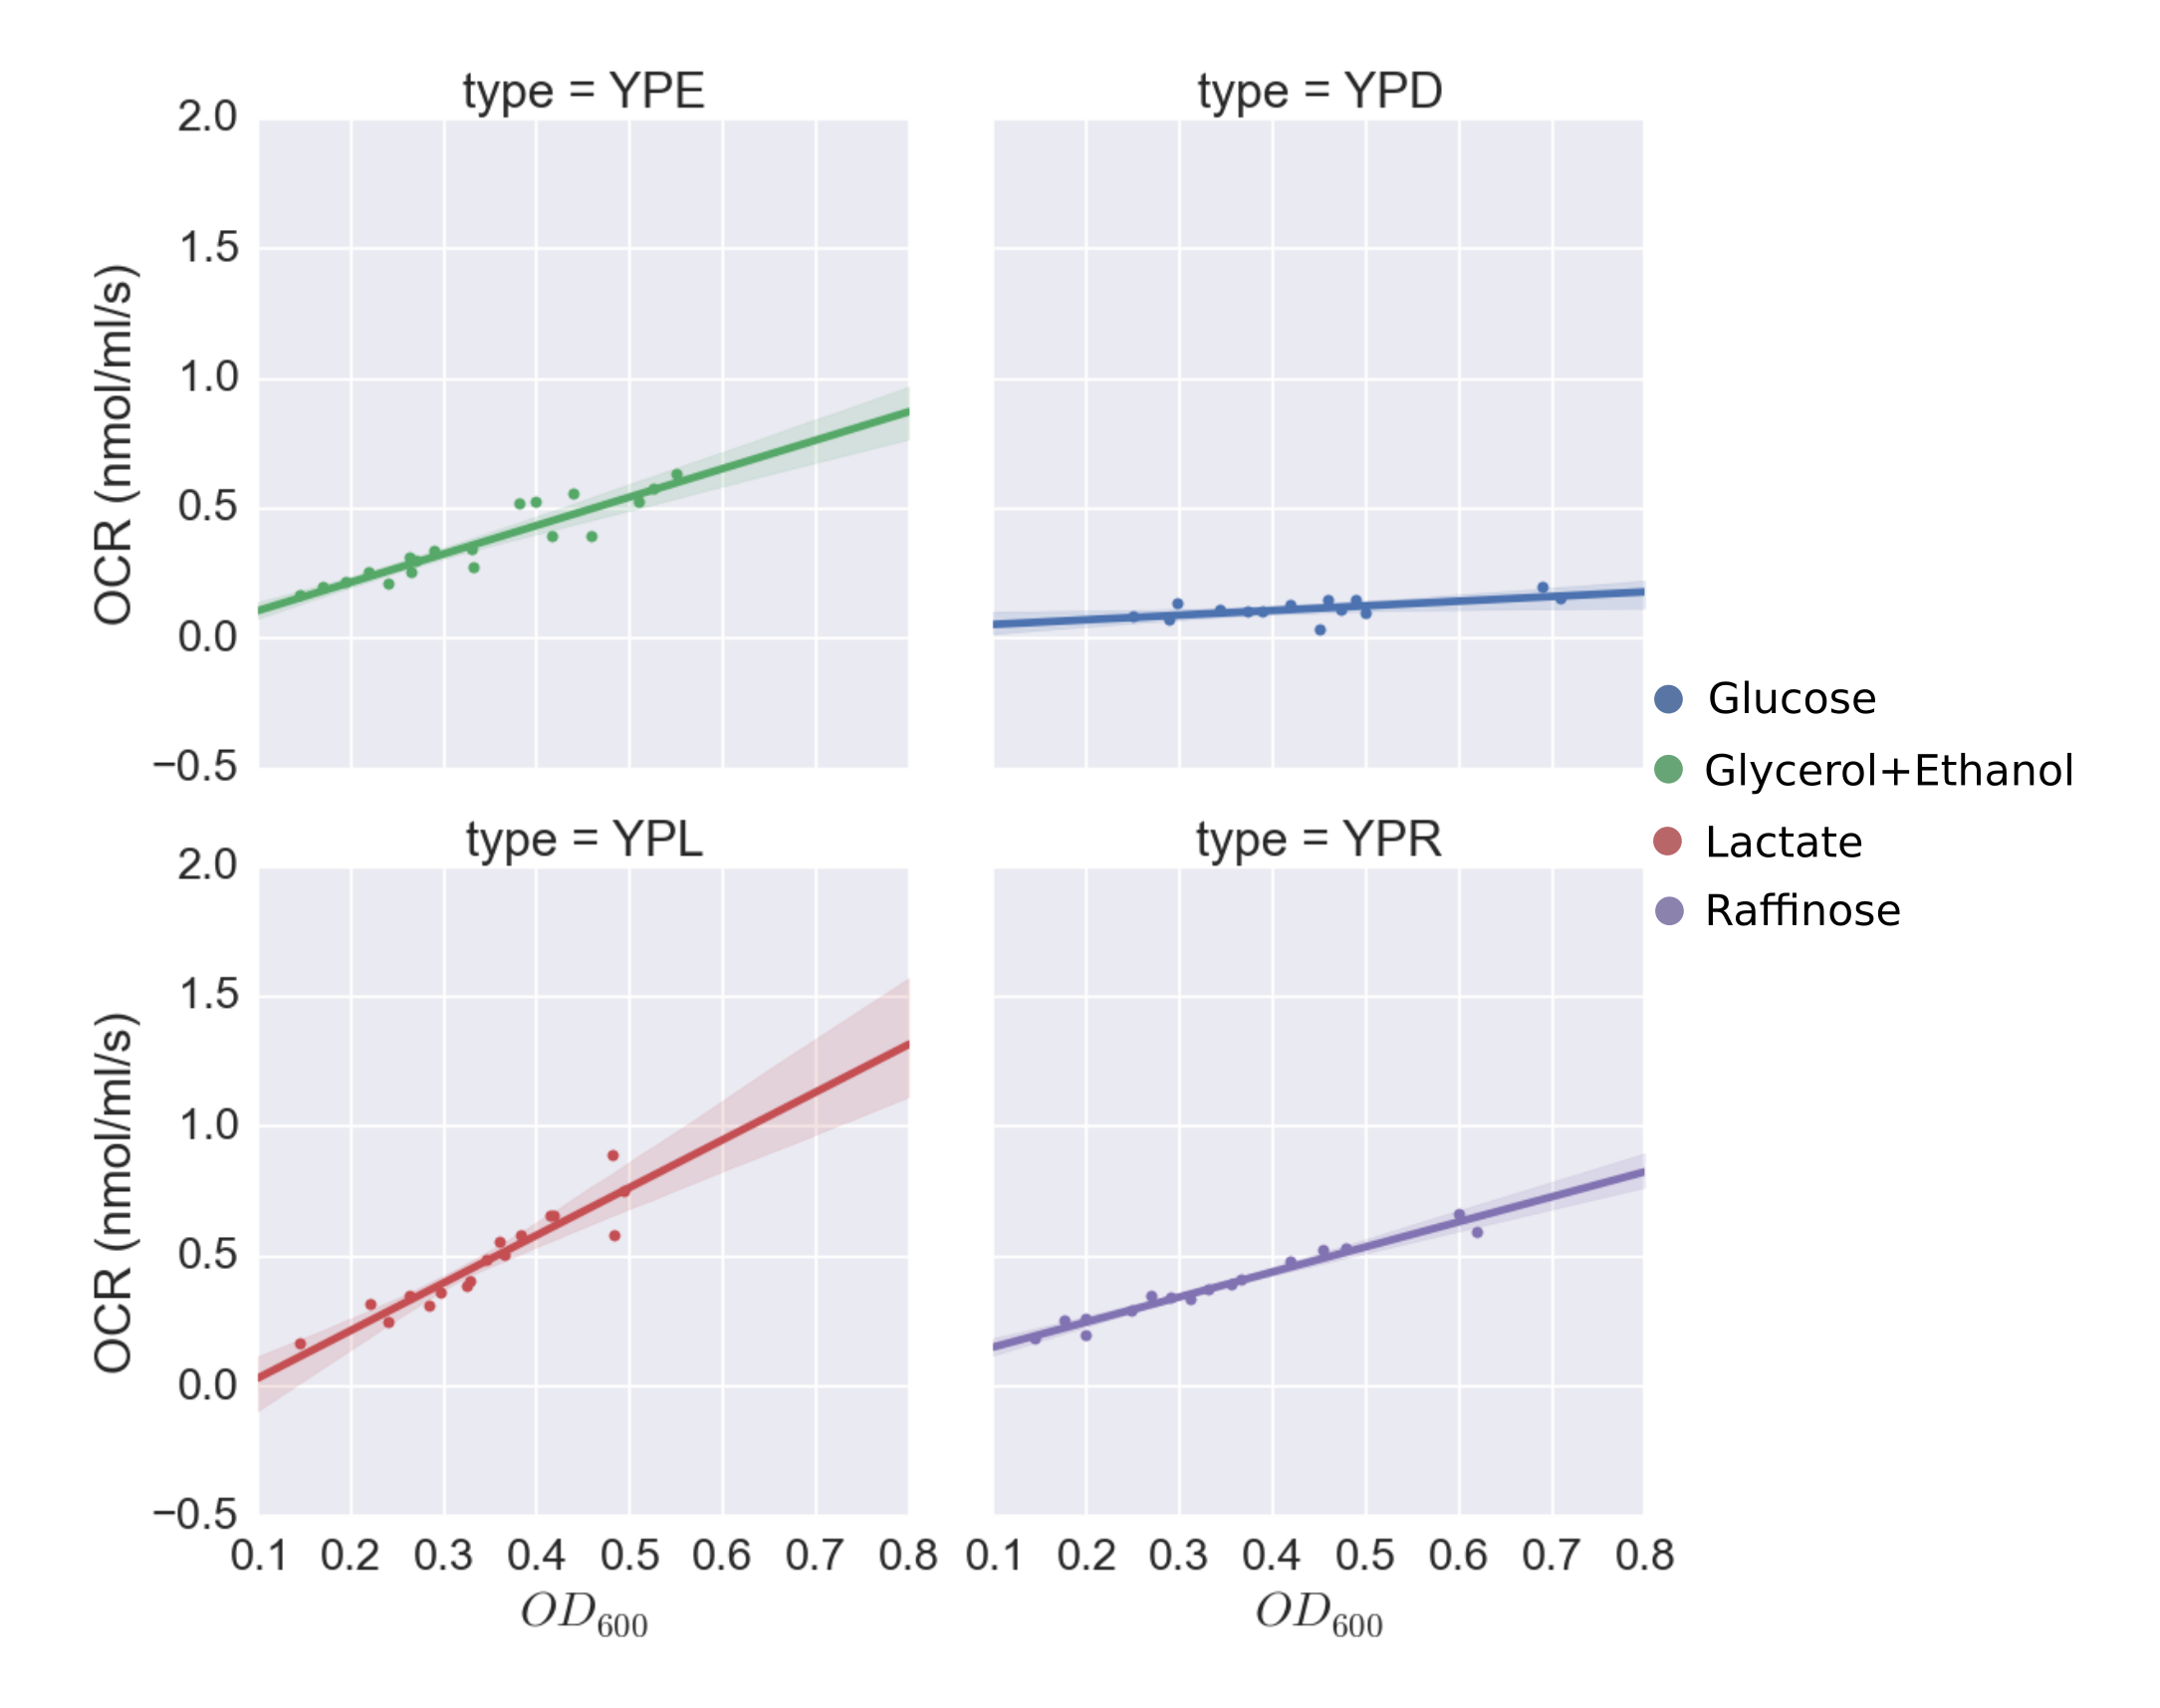
\includegraphics[width=\textwidth]{OCRraw}
    \caption[Respiration rate (OCR) as a function of optical density (OD$_{600}$).]{Respiration rate (OCR) as a function of optical density (OD$_{600}$).\\OCR readings from multiple sampling runs at different cell concentrations (OD$_{600}$) were plotted for cells grown in various carbon sources. The curve fit allows one to obtain the OCR at the OD$_{600}$=0.5 which we used as the standard OD reading to obtain normalized OCR by mass, cell number and mitochondrial volume.\\
\emph{Shaded band represent the bootstrapped 95\% confidence interval for the fitted values.}}\label{fig:OCRraw}
\end{figure}
%
%
\begin{figure}[htp]
	\centering
    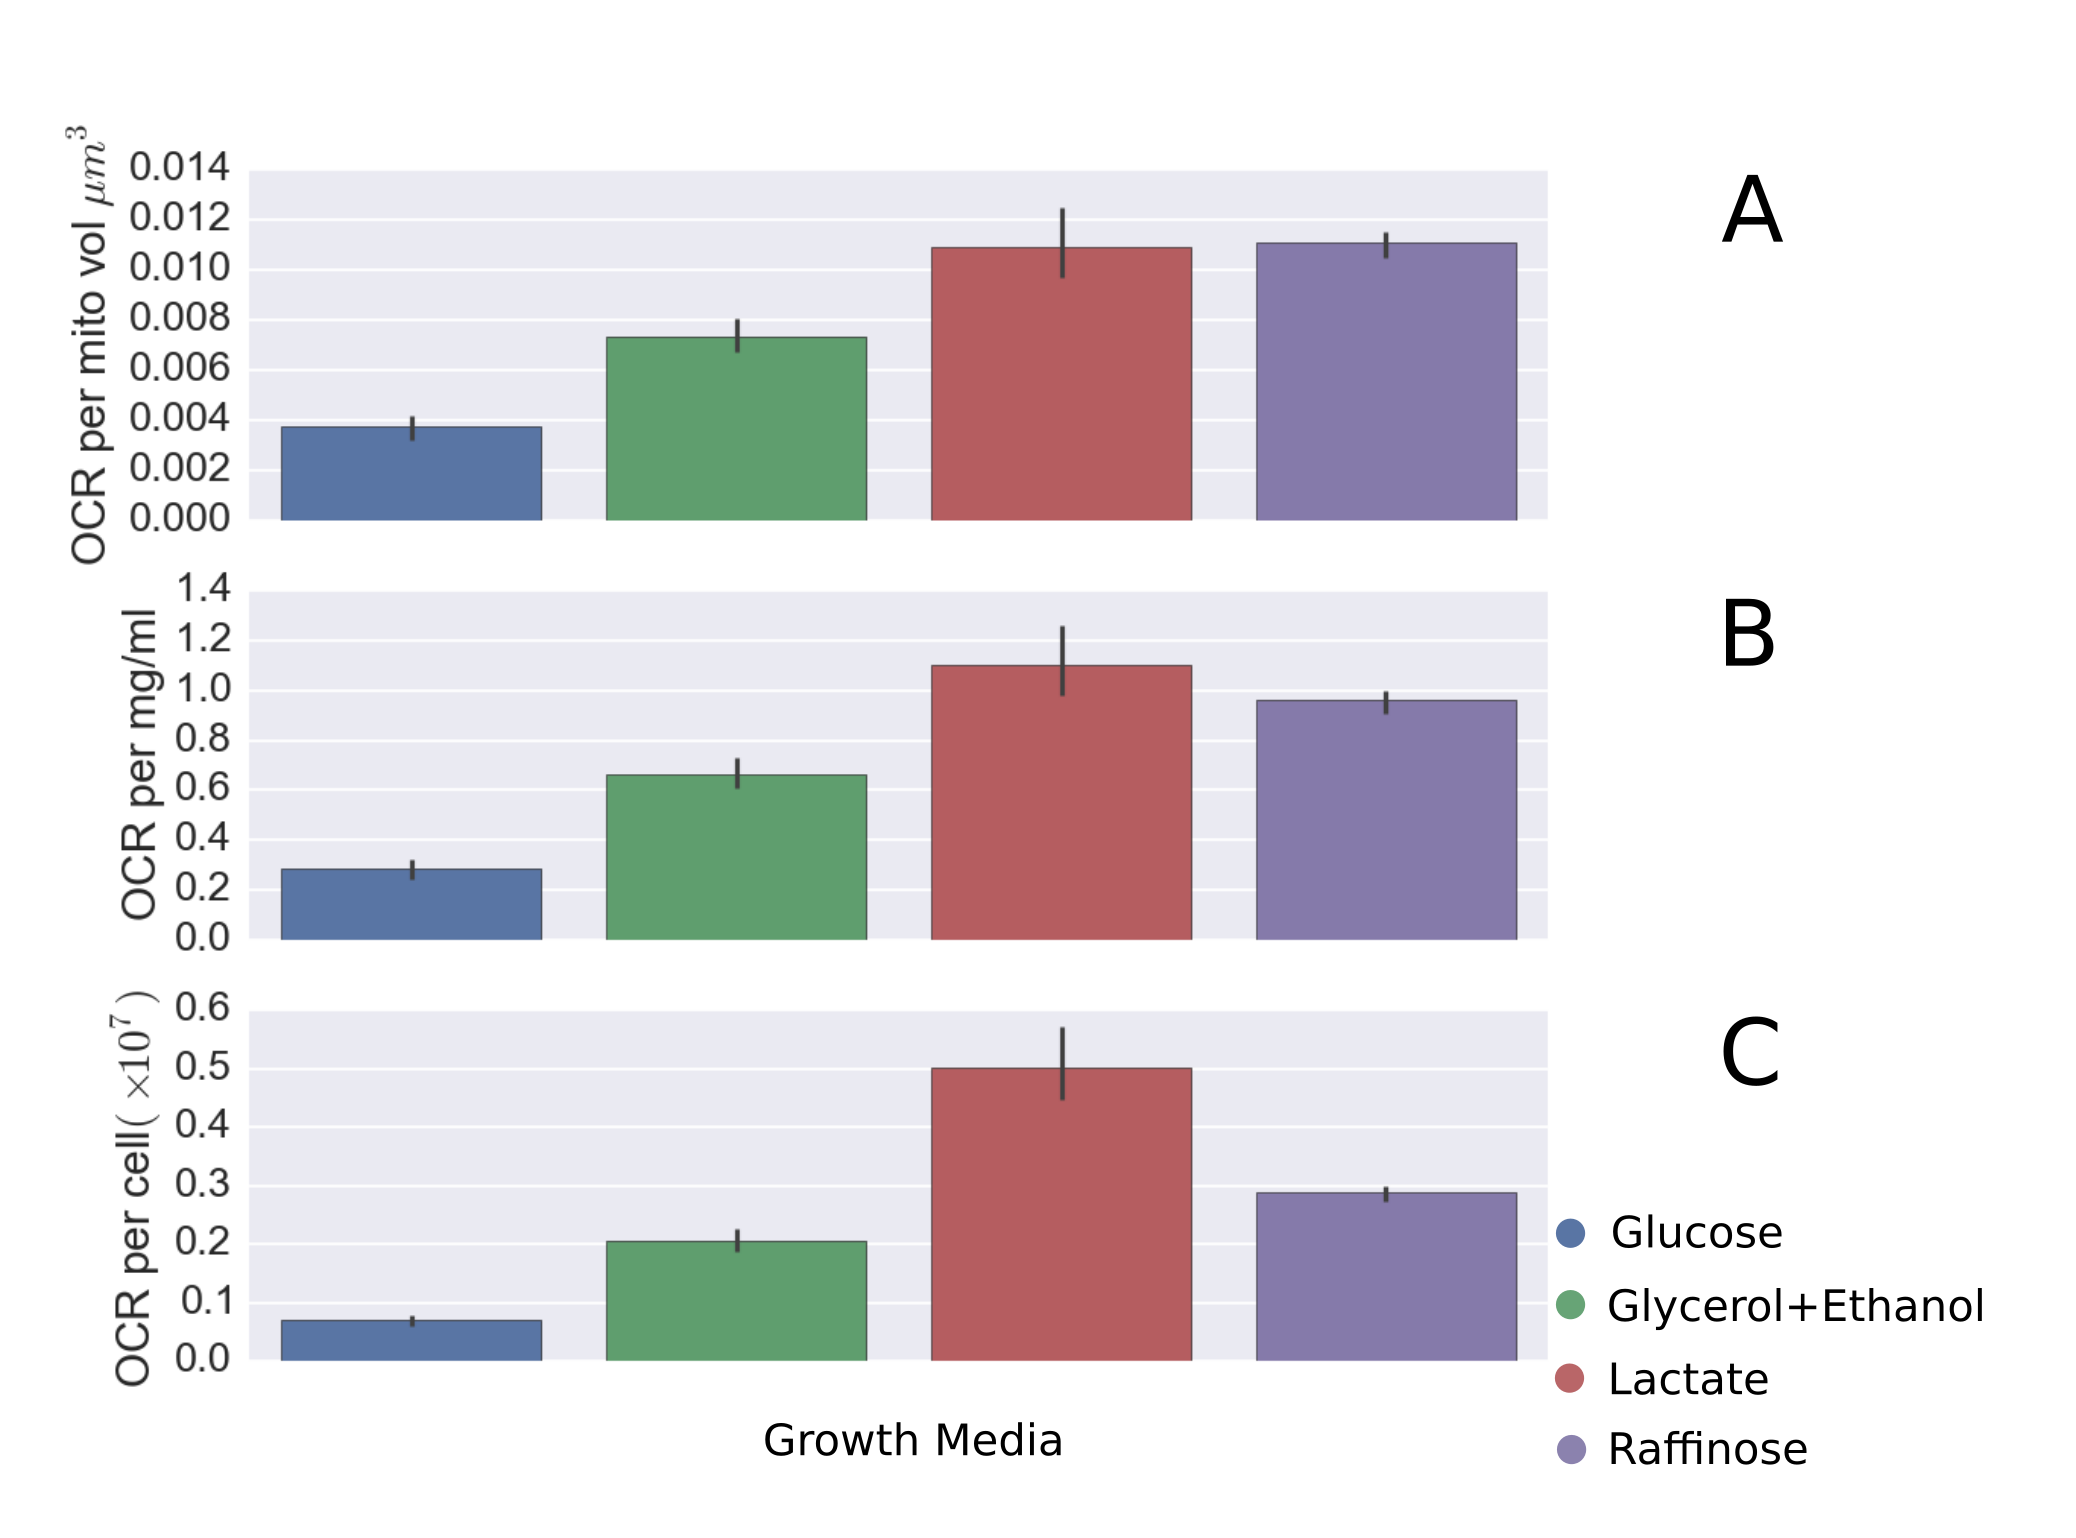
\includegraphics[width=\textwidth]{o2bars}
     \subcaptionbox{OCR normalized by mitochondrial volume\label{fig:O2barsA}}[\linewidth]{}
      \subcaptionbox{OCR normalized by dry mass\label{fig:O2barsB}}[\linewidth]{}
       \subcaptionbox{OCR normalized by number of cells\label{fig:O2barsC}}[\linewidth]{}
    \caption[Oxygen consumption rate (OCR) of yeast in different carbon sources.]{Oxygen consumption rate (OCR) of yeast in different carbon sources.\\OCR readings of yeast cells from sample volumes of 1 ml at OD$_{600}$=0.5 were normalized by mitochondrial volume (A), dry mass (B) or cell number (C). Different normalization methods result in different rankings of mitochondrial OCR in the different carbon sources. However mitochondria grown in glucose (fermentation condition) consistently showed the lowest mitochondrial OCR due to glucose repression. OCR normalized by mitochondrial volume is the most appropriate way to compare mitochondrial respiration rate as mitochondrial volume is a direct measurement of the amount of mitochondria in the sample volume. The other two methods scale not just with the amount of mitochondria in the sample volume but also cell size and numbers. OCR in glycerol+ethanol showed a two fold higher normalized OCR rate (\Fref{fig:O2barsA}) compared to glucose, while lactate and raffinose show a three fold higher normalized OCR rate compared to glucose.\\\emph{Error bars indicate the bootstrapped 95\% confidence interval of the median OCR value.}}\label{fig:O2bars}
\end{figure}
%
\section{Results}
We report OCR normalized in three different ways (\Fref{fig:O2bars}). \Fref{fig:O2barsA} shows the result of OCR in the different carbon conditions, normalized by mitochondrial volume. The other two subfigures show two standard ways OCR measurement in intact cells are usually reported in the literature, which are normalization by dry mass (\Fref{fig:O2barsB}) and cell number (\Fref{fig:O2barsC}). The OCR differences between the carbon conditions are similar regardless of the normalization methods except for the case of raffinose. In all cases glucose has the lowest OCR, lactate the highest and glycerol+ethanol intermediate between the two. Raffinose shows a respiration rate that is either similar to lactate (A and B) or lower than lactate but still higher than glycerol+ethanol. For the OCR normalized by mitochondrial volume measurements, cells grown in glycerol+ethanol showed a two fold increase in OCR levels compared to those in glucose (fermentation only conditions). Cells grown in lactate and raffinose show a three fold increase in OCR levels (lactate and raffinose had no significant difference in their OCR rate normalized to mitochondrial volume, evidenced by the error bars overlapping in \Fref{fig:O2barsA}).

We believe OCR normalized to total mitochondrial volume calculated from MitoGraph v2.0 is the most specific measure to show how mitochondrial respiration is affected by changes in growth conditions. Normalization by cell number does not account for changes in the proportion of the cell volume that is occupied by mitochondria (volume ratio) between different growth conditions. It cannot differentiate increased respiration due to there been more cells or because the cells have increased mitochondrial volume ratio. Normalizing by dry mass of cell also suffers from this problem; it cannot differentiate increased respiration due to there been more cells, and hence total mass or if specific cell mass increased due to increased mitochondrial volume ratio (or even if specific cell mass increased due to non mitochondrial content). An alternative OCR normalization method is normalizing by mitochondrial associated protein content.

The OCR levels for raffinose was surprising as we predicted it would be intermediate between the non-fermentable glycerol+ethanol and glucose substrates. Furthermore, ΔΨ levels did not correlate perfectly with OCR for the case of raffinose, glycerol+ethanol and lactate (\Fref{fig:O2dy}). Cells grown in glycerol+ethanol displayed the highest average ΔΨ level while having OCR intermediate between glucose and lactate/raffinose. These unexpected results are discussed further in the next section.
%
\begin{figure}[htp]
	\centering
    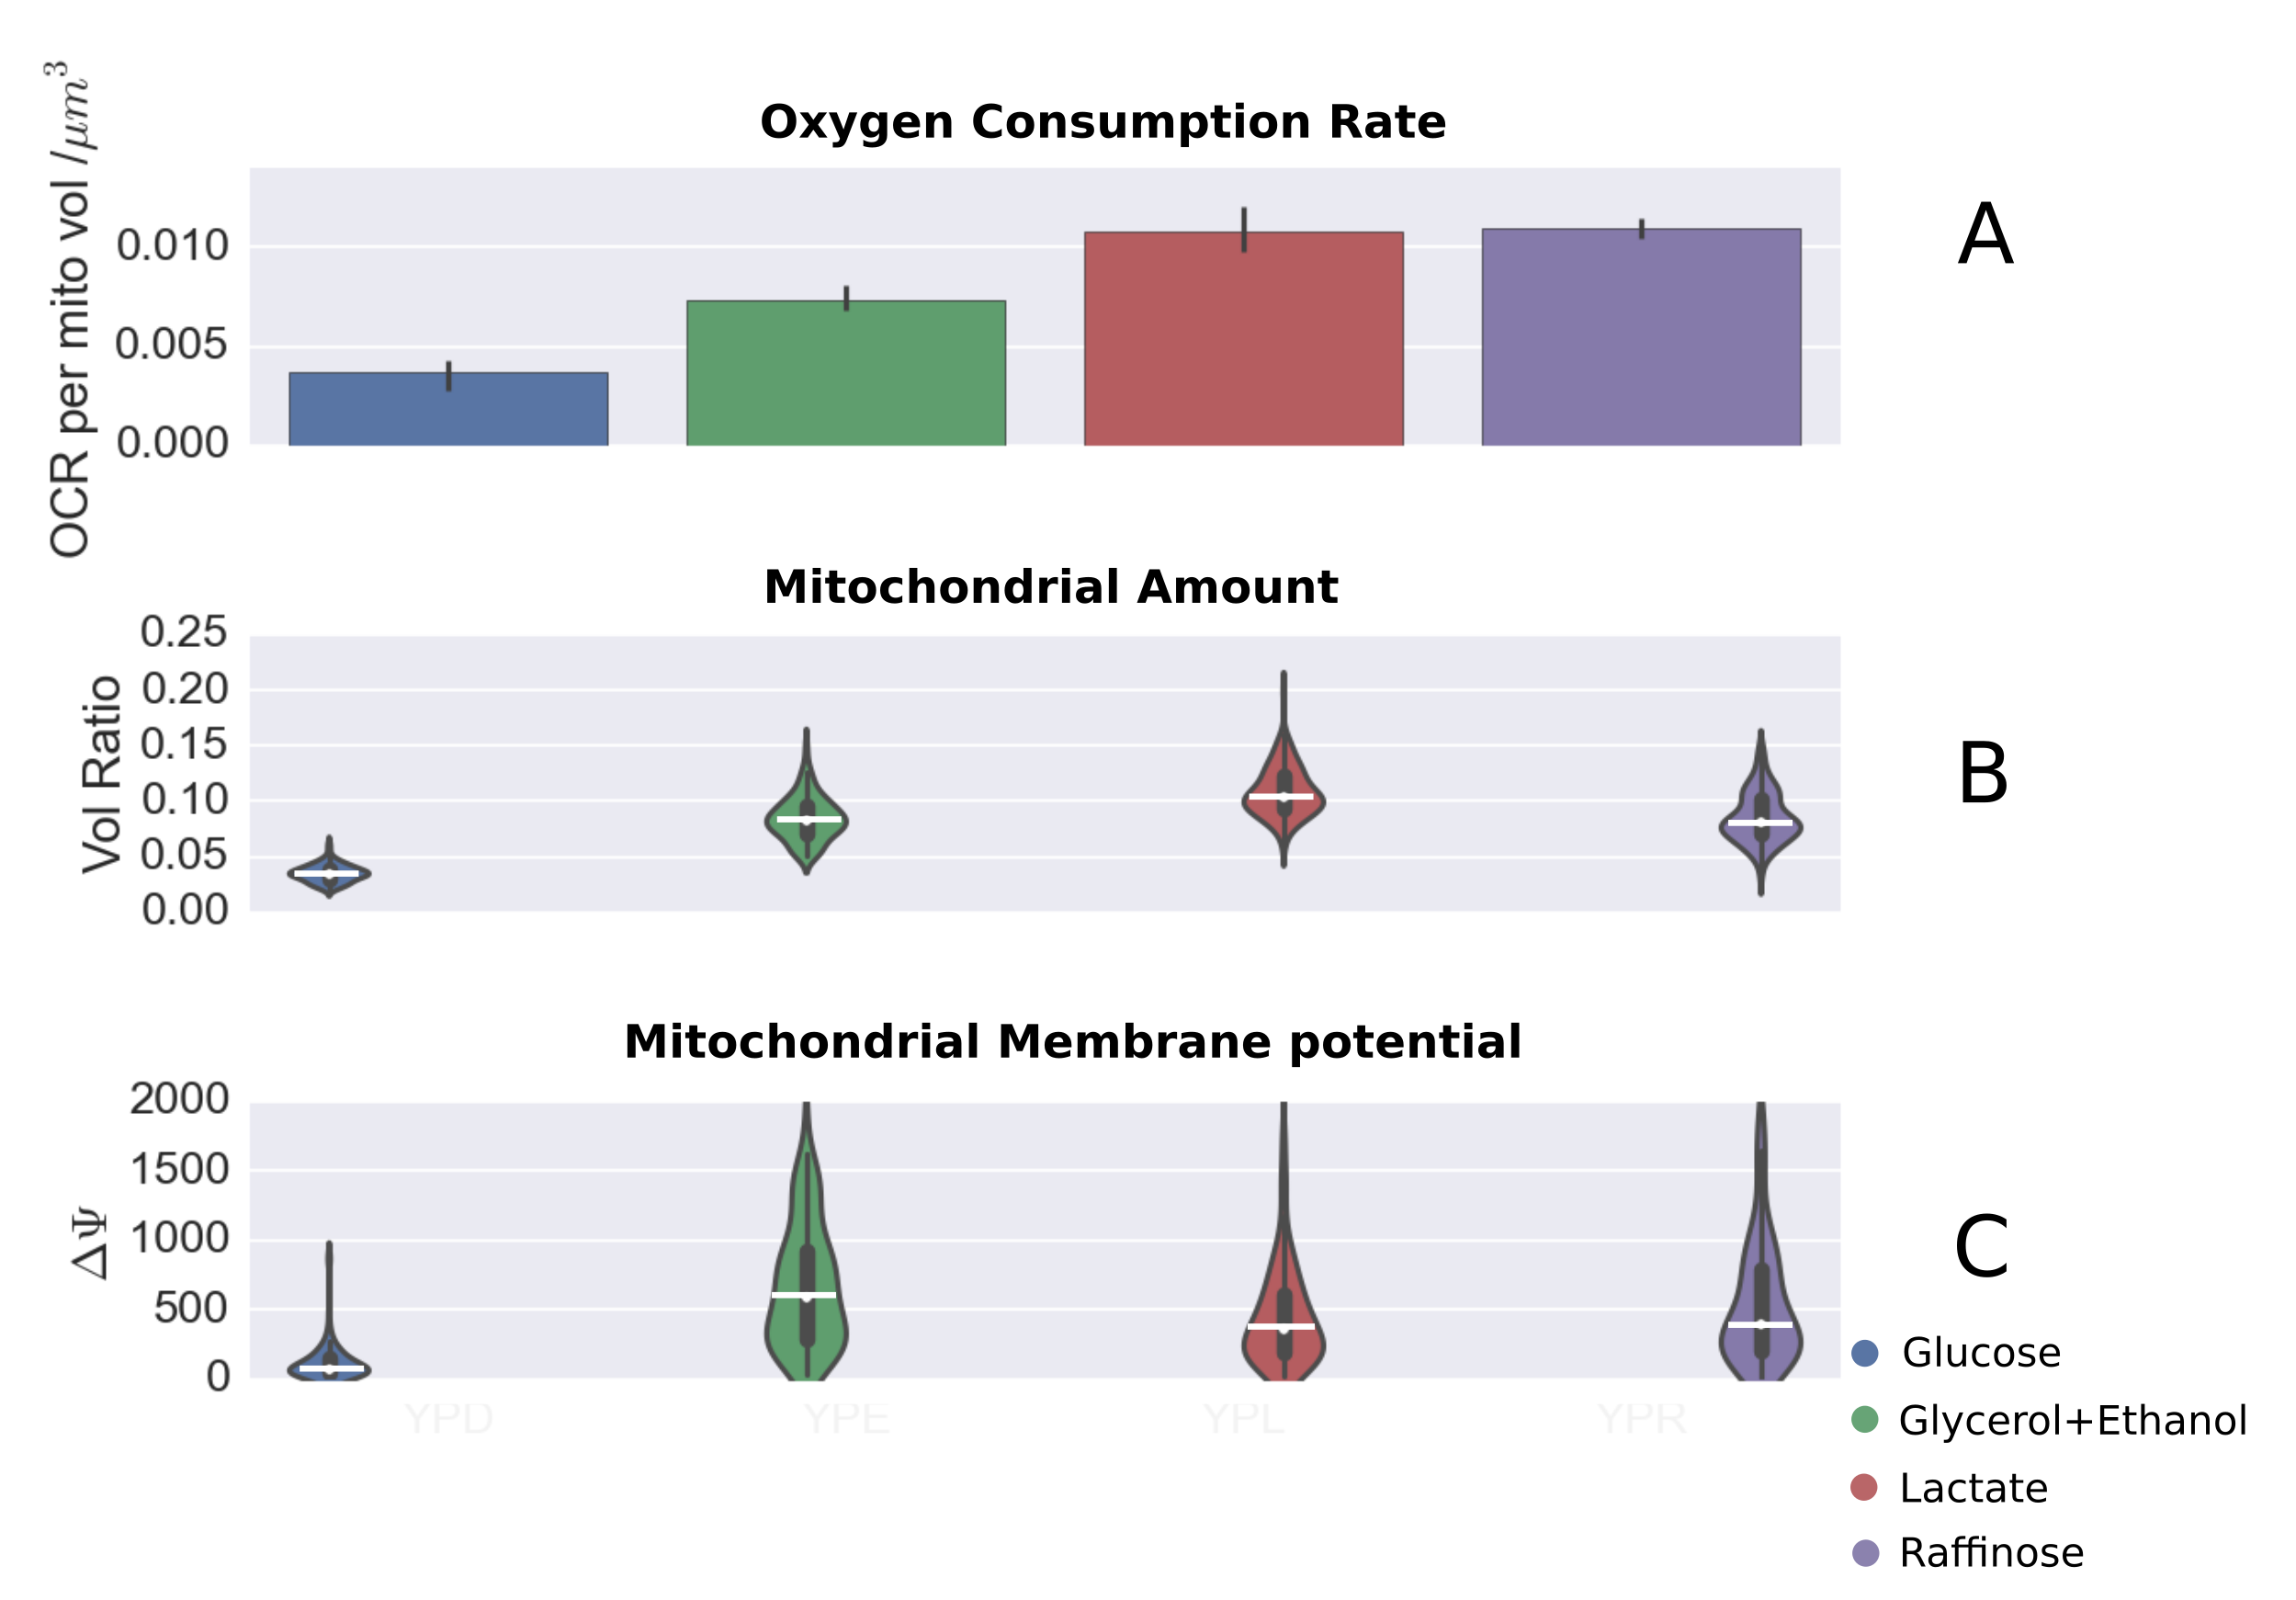
\includegraphics[width=\textwidth]{o2dy}
       \subcaptionbox{OCR normalized by mitochondrial volume\label{fig:O2dyA}}[\linewidth]{}
      \subcaptionbox{Mean volume ratio of population\label{fig:O2dyB}}[\linewidth]{}
       \subcaptionbox{Mean ΔΨ of population\label{fig:O2dyC}}[\linewidth]{}
    \caption[Relationship between mitochondrial OCR, membrane potential (ΔΨ) and amount density (volume ratio) of yeast grown in different carbon sources.]{The relationship between mitochondrial OCR, membrane potential (ΔΨ) and amount density (vol ratio) of yeast grown in different carbon sources.\\
Shown here is the relationship between mitochondrial OCR (A) and its relationship with the amount density of mitochondria in the cell (volume ratio, B) and ΔΨ (C). Mitochondria from cells grown in glycerol+ethanol display the highest ΔΨ levels and an intermediate respiration level, while those from cells grown in lactate display and intermediate level of ΔΨ and the highest respiration rate. We believe our results is due to lactate been oxidized less efficiently by the mitochondrial respiration machinery, hence the mitochondrial amount is increased in lactate to  compensate for a lesser cellular respiration efficiency. Raffinose displays similar levels of ΔΨ and respiration rates with lactate, while displaying a lower volume ratio of mitochondria. We believe that cellular respiration in raffinose is also less efficient that in glycerol+ethanol, but is able to maintain growth fitness by also undergoing fermentation.\\\emph{Error bars indicate the bootstrapped 95\% confidence interval of the median OCR value.\\White bars indicate median values.}}\label{fig:O2dy}
\end{figure}
%
\section{Discussion}
The literature has sparse references for basal OCR rate fold differences between yeast cells grown in different carbon sources under aerobic, exponential growth. Most studies used only one type of carbon condition (glucose) and therefore oxygen consumption rates are readily available for yeast grown in glucose \cite{meyenburg_energetics_1969}. One study measured the amount of basal respiration change as the amount of ethanol was slowly increased in yeast cells grown in glucose. They reported that respiration rate increased 50\% when ethanol concentration was at 2.5\%. However this was done on stationary phase (non proliferating) cells. Another study measured yeast grown in glucose repressing concentrations (2\%) and non respiration repressing concentrations (0.5\%) and found that respiration was increased two fold \cite{lin_calorie_2002}. No direct numbers could be found for basal OCR of yeast cells grown in glycerol, most likely because most often glycerol was considered as a byproduct of yeast metabolism rather than as a substrate in traditional yeast bioenergetic studies \cite{gancedo_glycerol_1968,wills_regulation_1990}. However according to one reference \cite{christopher_wills_effect_1984} only 10\% of the glycerol content is used by yeast grown on glycerol+ethanol. 

One study using lactate limited concentrations (0.2\%) reported OCR normalized to dry mass levels less than half of our results \cite{dejean_growth_2000}, but we caution that this result is not directly comparable as their growth media was substrate limiting, used a synthetic yeast nitrogen media without amino acids and had slower growth rate (doubling time 4 hrs vs 3.1 hrs). Lactate is oxidized to pyruvate by a \emph{lactate:cytochrome c} oxidoreductase complex and donates its electrons directly to cytochrome c, at the terminal end of the ETC. It has been reported that this serves as a shunt \cite{pajot_utilization_1974}, bypassing complex I, II and III. Thus because of the low proton motive force generated, one molecule of lactate only generates one ATP equivalent and hence lactate is a poor carbon source. Furthermore due to the fact that pyruvate oxidation can occur in the cytosol in yeast via the pyruvate dehydrogenase bypass \cite{boubekeur_mitochondrial_1999}, ATP yield is further reduced. Indeed it is known that the ATP/oxygen ratio of lactate is up to 50\% less than ethanol \cite{ohnishi_preparation_1966}. The high respiration reported here could be an indication that respiration is upregulated to make up for this poor ATP/oxygen ratio (known as coupling efficiency). Evidence for this is that in the previously mentioned study which used substrate limited concentrations of lactate (0.2\%), respiration rates were much less than our non substrate limited concentrations (2.0\%). However mitochondrial density is much higher than in glycerol+ethanol (\Fref{fig:O2dyB}), perhaps suggesting a compensatory upregulation of mitochondrial biogenesis to meet metabolic demands. Our growth rates for glycerol+ethanol and lactate are comparable (\textasciitilde2.9 hours for glycerol+ethanol vs 3.1 hrs for lactate, refer to growth curves in \Fref{fig:grwtcvs}), so there is evidence that cells grown in lactate have similar growth fitness with glycerol+ethanol even though lactate is a less efficient fuel source.

One study showed basal OCR levels around three fold higher in raffinose compared to glucose \cite{guaragnella_yeast_2013}, which is in good agreement with out results. However it is rather puzzling why raffinose which is considered to be able to undergo fermentation and respiration simultaneously would have a higher basal respiration rate compared to the non-fermentable carbon substrate glycerol+ethanol. One possibility is that high respiration levels seen in raffinose compared to glycerol+ethanol is due to high uncoupled respiration levels, which is further supported by the lower ΔΨ levels seen in raffinose compared to glycerol+ethanol (\Fref{fig:O2dyC}).

The best way to check whether respiration is less efficient in raffinose and lactate compared to in glycerol+ethanol is to measure respiratory control ratio (RCR). RCR is the ratio of the respiration levels at state 3 to state 4. A high RCR indicates a high level of respiration capacity with a low level of proton leak. Another similar parameter is the spare respiratory capacity, which is the difference between state 3 and basal respiration rate. This parameter indicates the capacity of the mitochondria to respond to an increase in energy demand. RCR is a complex function that depends on numerous factors such as the substrate given. Based on our hypothesis that mitochondrial respiration is less efficient in lactate and raffinose compared to glycerol+ethanol, we expect RCR values to be lower as well.

Measurement of RCR in yeast cells is problematic due to having to permeate the cell wall prior to addition of ETC chain inhibitors to achieve state 3 and 4 \cite{palmeira_fluorescence_2012}. Measurement of RCR using the Clark electrode is also difficult because the ability to add inhibitors to the sample during a measurement run is limited and multiple parallel experiments have to be conducted to obtain RCR parameters. We propose the use of the Seahorse system \cite{gerencser_quantitative_2009} to measure RCR. This system uses a piston to reversibly enclose a small volume (\textasciitilde \SI{2}{\ul}) above the cell layer. A probe containing a fluorophore is inserted into the chamber and measures the oxygen concentration by quenching of the fluorophore. The piston is then raised to allow the bulk media to reequilibrate. This system offers a convenient way to measure all the parameters related to cell respiration in one run, as up to four additions of inhibitors can be made per run.

Another possible reason that raffinose show lower respiration efficiency is that it might be somehow substrate limited. Certain common yeast lab strains lack the enzyme to metabolize melibiose, which is the form of glucose+galactose found in raffinose. However we found that our lab strain grew normally in melibiose (image data shown in \Fref{fig:meli}), therefore the yeast cells we used grown in raffinose were not substrate limited.